\section{Aufbau und Durchführung}
\subsection{Aufbau}
\label{sec:Aufbau}

Der Franck-Hertz-Versuch, Abbildung \ref{lel}, wird in einer Röhre durchgeführt, in der sich zwei Elektroden sowie ein Glühdraht befinden.
Der Glühdraht, auf dem eine konstante Heizspannung gegeben wird, dient durch den auftretenden glühelektrischen Effekt als Elektronenquelle.
Hierzu wird ein Metall mit einem hohen Schmelzpunkt, beispielsweise Wolfram, verwendet, so dass eine Elektronenwolke entsteht.
Diese Elektronen werden zu einer gitterförmigen Beschleunigungselektrode beschleunigt, welche sich in der Mitte der Röhre befindet.
Durch Wahl einer passenden Beschleunigungsspannung $U_B$ kann die Energiezufuhr der Elektronen gesteuert werden.
Am Ende des Gefäßes befindet sich zudem eine Auffängerelektrode, welche die Elektronen durch eine zwischen der Beschleunigungs- und Auffängerelektrode anliegenden Spannung $U_A$ abbremst.
Die Anzahl der auftreffenden Elektronen kann mithilfe eines Picoamperemeters anhand des Auffängerstroms $I_A$ bestimmt werden.
Dieses Messgerät verstärkt und wandelt den geringen Eingangsstrom um, so dass dieser als Spannung auf die Y-Achse eines XY-Schreibers gegeben werden kann.
Durch das zusätzliche Anlegen von $U_A$ oder $U_B$ am X-Eingang wird somit der Eingangsstrom in Abhängigkeit einer variablen Beschleunigungs- oder Bremsspannung graphisch dargestellt.
\\

Zudem ist in der evakuierten Röhre eine geringe Menge Quecksilber platziert, welches je nach gewählter Umgebungstemperatur $T$ einen variablen Dampfdruck $p_\text{sät}$ besitzt.
Die Temperatur wird mittels eines elektronischen Temperaturreglers geregelt und anhand eines zusätzlich angebrachten Thermometers kontrolliert.

\begin{figure}[H]
  \centering
  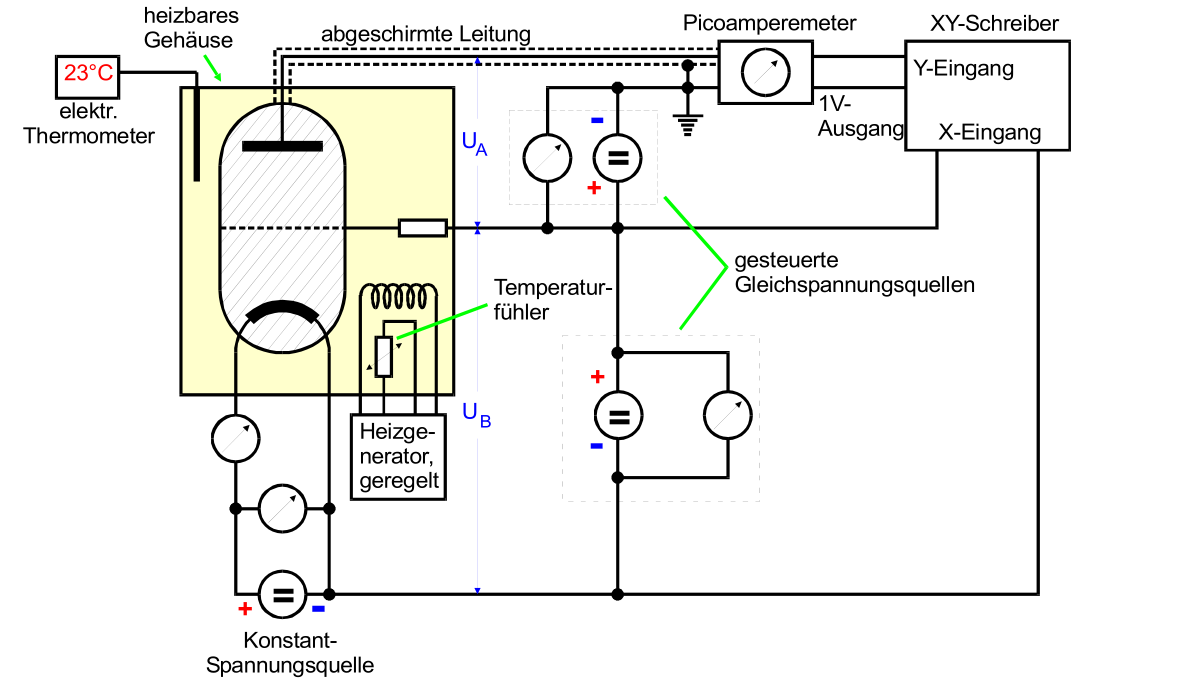
\includegraphics[height=6cm]{ressources/aufbau2.png}
  \caption{Aufbau des Franck-Hertz-Versuchs. \cite{skript}}
  \label{lel}
\end{figure}
